\documentclass[10pt,a4paper]{article}
\usepackage[UTF8,fontset = windows]{ctex}
\setCJKmainfont[BoldFont=黑体,ItalicFont=楷体]{华文中宋}
\usepackage{amssymb,amsmath,amsfonts,amsthm,mathrsfs,dsfont,graphicx}
\usepackage{ifthen,indentfirst,enumerate,color,titletoc}
\usepackage{tikz}
\usepackage{multicol}
\usepackage{makecell}
\usepackage{longtable}
\usetikzlibrary{arrows,calc,intersections,patterns,decorations.pathreplacing,3d,angles,quotes,positioning}
\usepackage[bf,small,indentafter,pagestyles]{titlesec}
\usepackage[top=1in, bottom=1in,left=0.8in,right=0.8in]{geometry}
\renewcommand{\baselinestretch}{1.65}
\newtheorem{defi}{定义~}
\newtheorem{eg}{例~}
\newtheorem{ex}{~}
\newtheorem{rem}{注~}
\newtheorem{thm}{定理~}
\newtheorem{coro}{推论~}
\newtheorem{axiom}{公理~}
\newtheorem{prop}{性质~}
\newcommand{\blank}[1]{\underline{\hbox to #1pt{}}}
\newcommand{\bracket}[1]{(\hbox to #1pt{})}
\newcommand{\onech}[4]{\par\begin{tabular}{p{.9\textwidth}}
A.~#1\\
B.~#2\\
C.~#3\\
D.~#4
\end{tabular}}
\newcommand{\twoch}[4]{\par\begin{tabular}{p{.46\textwidth}p{.46\textwidth}}
A.~#1& B.~#2\\
C.~#3& D.~#4
\end{tabular}}
\newcommand{\vartwoch}[4]{\par\begin{tabular}{p{.46\textwidth}p{.46\textwidth}}
(1)~#1& (2)~#2\\
(3)~#3& (4)~#4
\end{tabular}}
\newcommand{\fourch}[4]{\par\begin{tabular}{p{.23\textwidth}p{.23\textwidth}p{.23\textwidth}p{.23\textwidth}}
A.~#1 &B.~#2& C.~#3& D.~#4
\end{tabular}}
\newcommand{\varfourch}[4]{\par\begin{tabular}{p{.23\textwidth}p{.23\textwidth}p{.23\textwidth}p{.23\textwidth}}
(1)~#1 &(2)~#2& (3)~#3& (4)~#4
\end{tabular}}
\begin{document}

\begin{enumerate}[1.]

\item { (003815)}在同一坐标系中画出函数$y=\log_a x, \ y=a^x, y=x+a$的图像, 可能正确的是\blank{30}.
\fourch{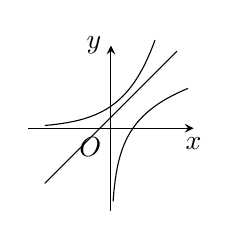
\begin{tikzpicture}[>=stealth,samples=100, scale = 0.7]
\draw [->] (-1.5,0)--(0,0) node [below left] {$O$}--(1.5,0) node [below] {$x$};
\draw [->] (0,-1.5)--(0,1.5) node [left] {$y$};
\draw [domain=-3:3] plot ({\x*0.4},{(\x+0.5)*0.4});
\draw [domain=-3:2] plot ({\x*0.4},{exp(\x*ln(2))*0.4});
\draw [domain=0.1:3.5] plot ({\x*0.4},{ln(\x)/ln(2)*0.4});
\end{tikzpicture}}{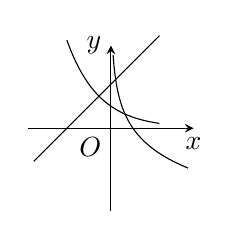
\begin{tikzpicture}[>=stealth,samples=100, scale = 0.7]
\draw [->] (-1.5,0)--(0,0) node [below left] {$O$}--(1.5,0) node [below] {$x$};
\draw [->] (0,-1.5)--(0,1.5) node [left] {$y$};
\draw [domain=-3.5:2.2] plot ({\x*0.4},{(\x+2)*0.4});
\draw [domain=-2:2.2] plot ({\x*0.4},{exp(\x*ln(1/2))*0.4});
\draw [domain=0.1:3.5] plot ({\x*0.4},{-ln(\x)/ln(2)*0.4});
\end{tikzpicture}}{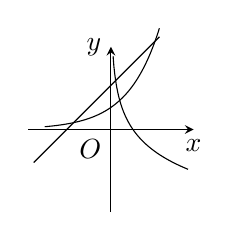
\begin{tikzpicture}[>=stealth,samples=100, scale = 0.7]
\draw [->] (-1.5,0)--(0,0) node [below left] {$O$}--(1.5,0) node [below] {$x$};
\draw [->] (0,-1.5)--(0,1.5) node [left] {$y$};
\draw [domain=-3.5:2.2] plot ({\x*0.4},{(\x+2)*0.4});
\draw [domain=-3:2.2] plot ({\x*0.4},{exp(\x*ln(2))*0.4});
\draw [domain=0.1:3.5] plot ({\x*0.4},{-ln(\x)/ln(2)*0.4});
\end{tikzpicture}}{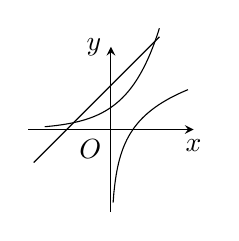
\begin{tikzpicture}[>=stealth,samples=100, scale = 0.7]
\draw [->] (-1.5,0)--(0,0) node [below left] {$O$}--(1.5,0) node [below] {$x$};
\draw [->] (0,-1.5)--(0,1.5) node [left] {$y$};
\draw [domain=-3.5:2.2] plot ({\x*0.4},{(\x+2)*0.4});
\draw [domain=-3:2.2] plot ({\x*0.4},{exp(\x*ln(2))*0.4});
\draw [domain=0.1:3.5] plot ({\x*0.4},{ln(\x)/ln(2)*0.4});
\end{tikzpicture}}


关联目标:

K0209003B|D02002B|会根据函数定义域, 利用计算器合理采点, 并能通过描点法作出指数函数$y=2^{x}$, $y=3^{x}$, $y=(1/2)^{x}$的大致图像.

K0210002B|D02002B|知道指数函数图像过定点$(0,1)$.

K0212003B|D02002B|会根据函数定义域, 利用计算器合理采点, 并能通过描点法作出对数函数$y=\log_2x,y=\log_3x,y=\log_{1/2}x$的大致图像.

K0213002B|D02002B|知道对数函数的图像过定点$(1,0)$.



标签: 第二单元

答案: 暂无答案

解答或提示: 暂无解答与提示

使用记录:

暂无使用记录


出处: 2016年双基百分百
\end{enumerate}



\end{document}